\section{Trondheim 3D: learning CesiumJS}\label{sec:p2}

\subsection{Purpose}

CesiumJS \citep{cesiumjs} is one of the most widely used libraries for 3D maps and digital globes on the web, and I wanted to learn it properly. The best way seemed to be to build something real in a place I know: a 3D model of Trondheim with terrain, buildings and one open dataset. I chose DSB's register of public shelters (\emph{tilfluktsrom}), because it raises a simple, practical question: which shelter is closest, and how far is the walk?

\subsection{What I built}

\begin{itemize}
  \item A full-screen 3D view of Trondheim with Cesium World Terrain and Cesium OSM Buildings (\cref{fig:p2-overview}).
  \item The public shelters as points on the map. Clicking one shows its number, capacity and address.
  \item A control panel with preset camera views (Midtbyen, Nidarosdomen, Bakklandet) and layer switches, which turns into a bottom sheet on phones.
  \item ``Nearest shelter'': click the ground, and the app finds the nearest shelter along the OpenStreetMap walking network and draws the route (\cref{fig:p2-route}).
\end{itemize}

\begin{figure}[htbp]
\centering
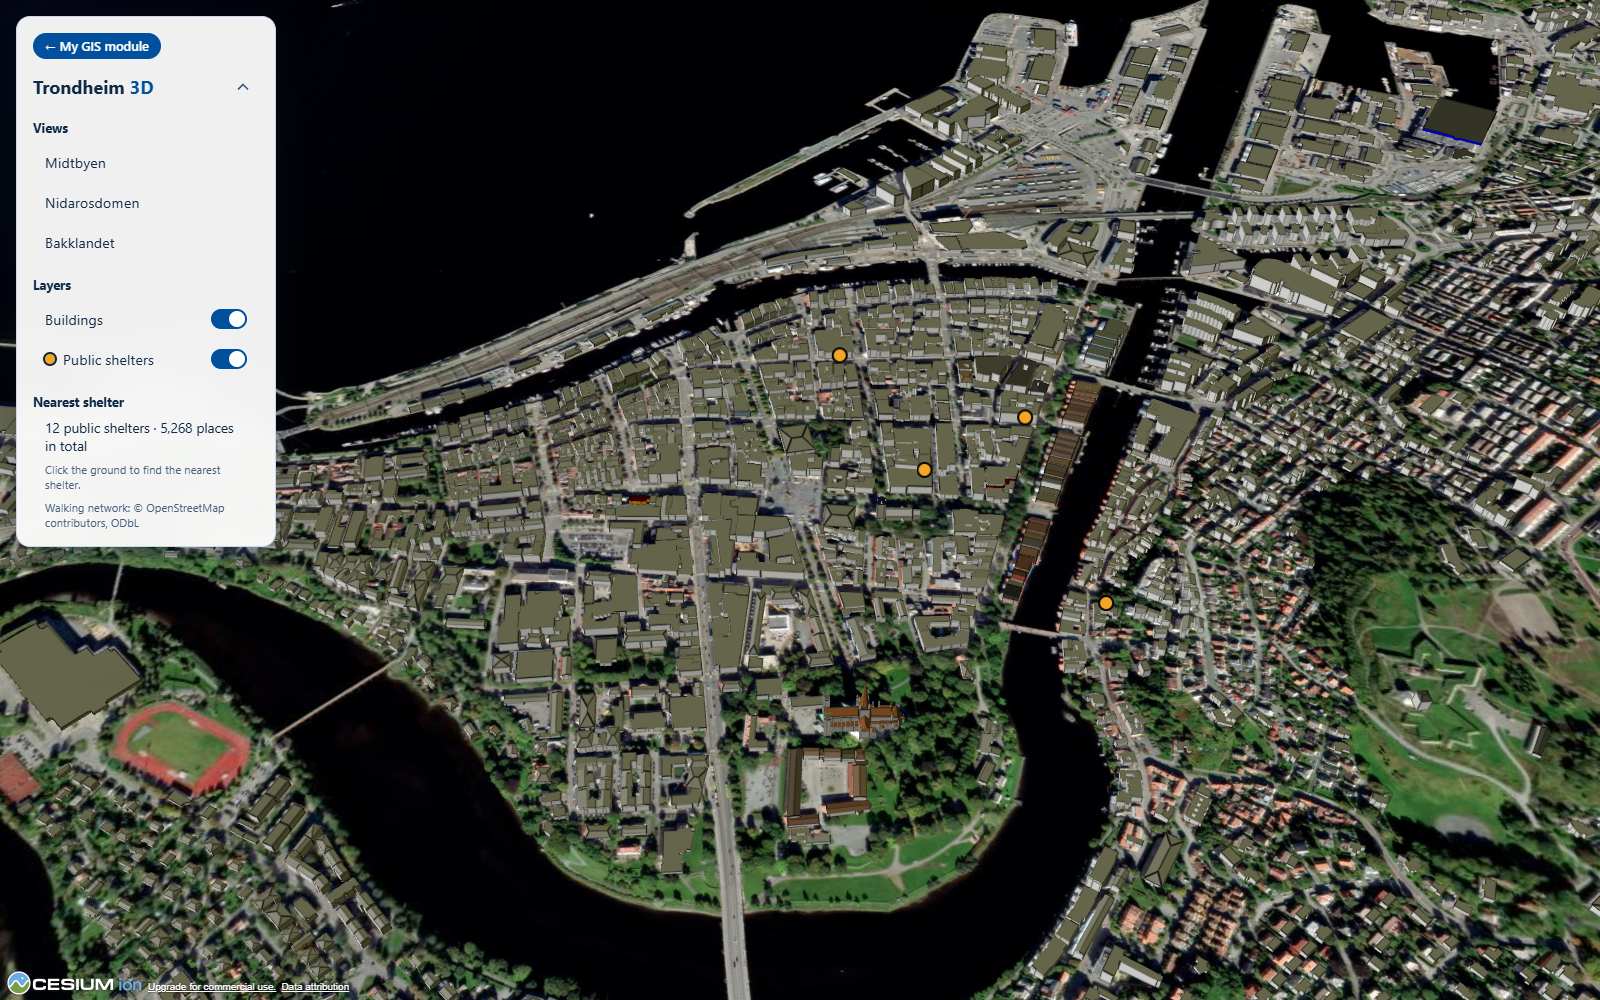
\includegraphics[width=\textwidth]{project-2-01-midtbyen-buildings.png}
\caption{Trondheim 3D: OpenStreetMap buildings on Cesium World Terrain, with the public shelters as orange points. Data: \textcopyright{} OpenStreetMap contributors (ODbL); Cesium ion; \textcopyright{} DSB (NLOD 2.0).}
\label{fig:p2-overview}
\end{figure}

\subsection{What I learned about CesiumJS}

\paragraph{The Viewer and Cesium ion.} Everything starts with a \code{Viewer}, which brings a globe, a camera and default imagery. Terrain and buildings are streamed from Cesium ion, which needs an access token. Because a web app's code is public, the token is visible to anyone; I learned to use a separate production token that only works from my own website.

\paragraph{3D Tiles.} The buildings are Cesium OSM Buildings, streamed as 3D Tiles \citep{3dtiles}: the city is split into tiles at several levels of detail, and Cesium loads finer tiles only where the camera needs them. One setting, \code{maximumScreenSpaceError}, controls this trade-off. I tested a coarser value to save memory, but small buildings in the centre disappeared, so I kept the default.

\paragraph{Entities, primitives and picking.} The shelters are \emph{entities} loaded from GeoJSON, which come with built-in selection and an info box. The buildings are a \emph{primitive}, the lower-level and faster way to draw large data. Picking showed the difference in practice: a click on a building or shelter selects that object, while a click on the ground returns a position on the terrain, which starts the nearest-shelter search.

\paragraph{The camera.} My first preset views used guessed camera positions and missed their landmarks. The fix was to describe each view as a target point plus a direction and a distance, and let Cesium place the camera in the target's local east-north-up frame. Then the landmark is always centred.

\paragraph{Using Cesium with React.} I kept Cesium code outside React components, in small modules for each layer, and gave every layer its own error handling, so the rest of the app keeps working if one dataset fails to load.

\subsection{What I learned about Norwegian geodata}

The shelters are published by DSB through an OGC Web Feature Service \citep{ogcwfs} in EUREF89 / UTM zone 32N (EPSG:25832), so they had to be converted to longitude and latitude for Cesium. Heights were the bigger lesson. Cesium measures heights above the WGS~84 ellipsoid, while Norwegian heights (NN2000) are measured above the geoid, which lies about 40\,m higher in Trondheim. Mixing the two puts a point about 40\,m too low. The walking network came from OpenStreetMap through the Overpass API \citep{overpass}.

\subsection{The nearest-shelter analysis}

Instead of a routing service, whose API key would be public in the browser, the app downloads the walking network once and searches it with Dijkstra's algorithm \citep{dijkstra1959}, directly in the browser. \Cref{fig:p2-route} shows why this matters: the nearest shelter is 490\,m away in a straight line, but the river is in the way, and the walk over Gamle Bybro is 684\,m. The analysis is simple, though: it ignores hills, stairs and how many people each shelter can take.

\begin{figure}[htbp]
\centering
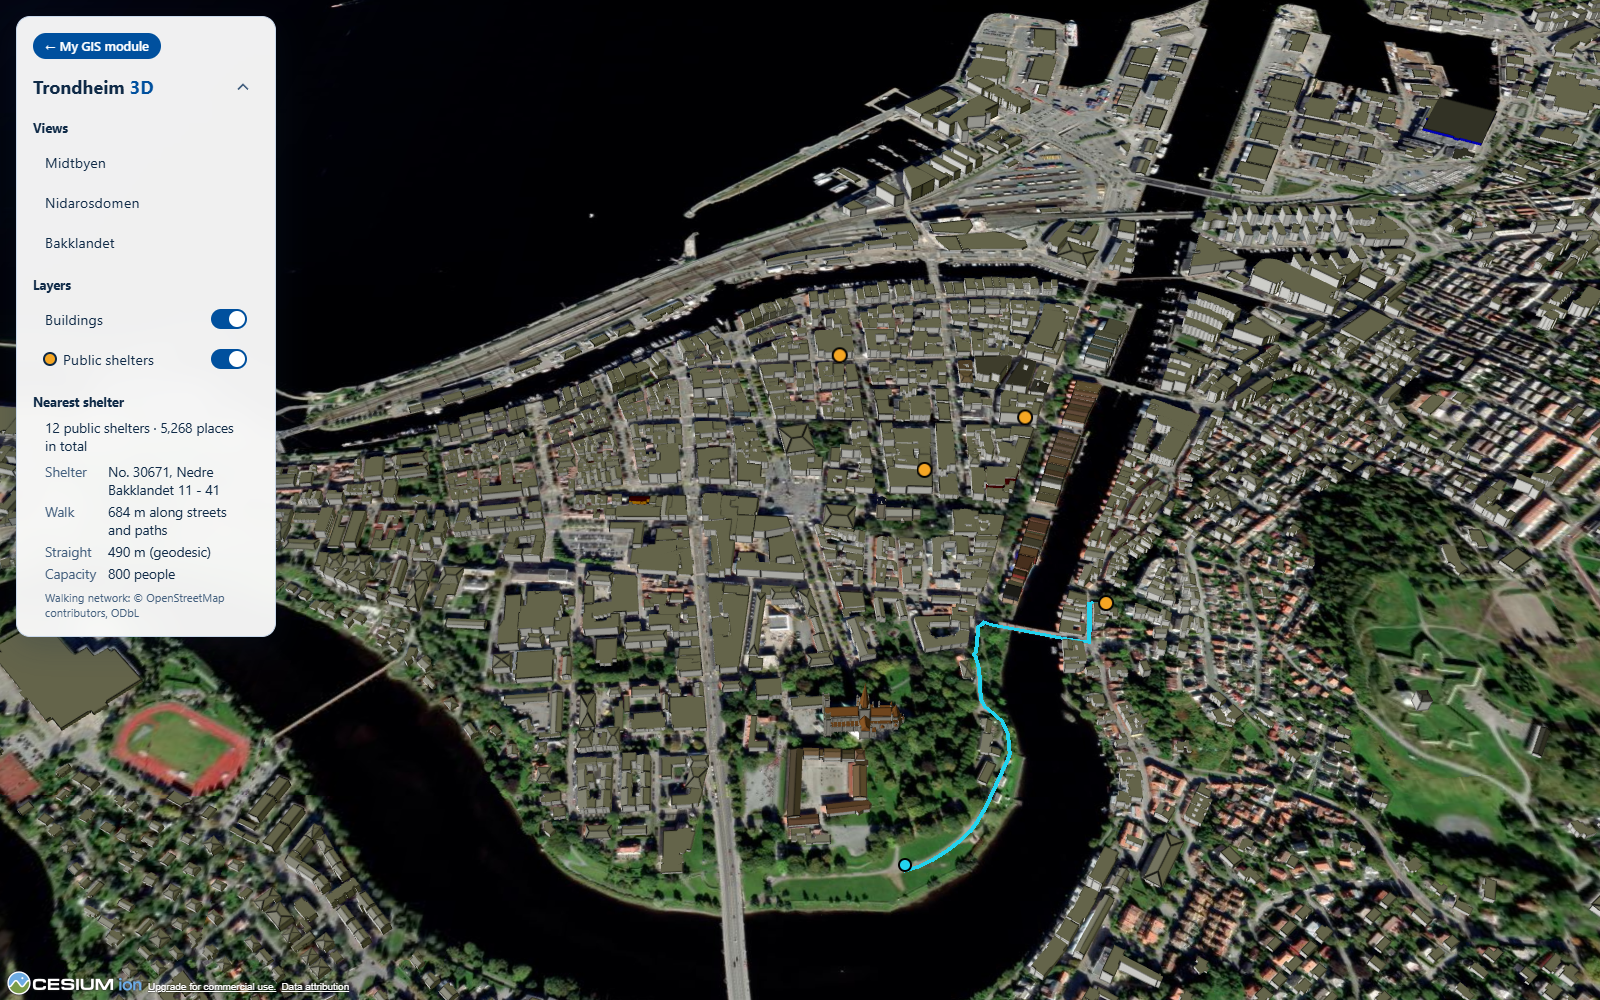
\includegraphics[width=\textwidth]{project-2-03-nearest-shelter-route.png}
\caption{A click south of Nidarosdomen: the nearest shelter is 490\,m away in a straight line, but the walk across the river is 684\,m. Data: \textcopyright{} DSB (NLOD 2.0); \textcopyright{} OpenStreetMap contributors (ODbL); Cesium ion.}
\label{fig:p2-route}
\end{figure}
